\chapter{Elektronegativiteit, polariteit en krachten tussen moleculen}\label{ch:g11:polarity-and-cohesion}

Een gekko rent tegen een ruit op en hangt aan één teen aan het glas,
zonder lijm en zonder zuignap. Een watermolecuul, \ce{H2O}, is lichter
dan een \omterm{def:g7:atoms-and-molecules:molecule}{molecuul} waterstofsulfide, \ce{H2S}, en toch kookt water bij
\qty{100}{\celsius}, terwijl waterstofsulfide tot
\qty{-60}{\celsius} een gas is. Beide verhalen gaan over hetzelfde: de
krachten die \omterm{def:g7:atoms-and-molecules:molecule}{moleculen} bij elkaar houden, en aan andere dingen. Ze zijn
veel zwakker dan de \omterm{def:g10:lewis-and-shape:covalent-bond}{covalente bindingen} binnen een \omterm{def:g7:atoms-and-molecules:molecule}{molecuul}, maar ze
bepalen of een stof bij kamertemperatuur een gas, een vloeistof of een
vaste stof is, en of een gekko valt.

\begin{recall}
Een \omterm{def:g10:lewis-and-shape:covalent-bond}{covalente binding} is een elektronenpaar dat door twee \omterm{def:g7:atoms-and-molecules:atom}{atomen} gedeeld
wordt; \omterm{def:g10:lewis-and-shape:lewis-structure}{lewisstructuren} tonen bindende en \omterm{def:g10:lewis-and-shape:lone-pair}{vrije elektronenparen}, en de
paren rond een centraal \omterm{def:g7:atoms-and-molecules:atom}{atoom} bepalen de vorm van een \omterm{def:g7:atoms-and-molecules:molecule}{molecuul}
(\cref{ch:g10:lewis-and-shape}). \omterm{def:g9:ions:ion}{Ionen} dragen een lading; in een
ionaire vaste stof trekken positieve en negatieve \omterm{def:g9:ions:ion}{ionen} elkaar aan
(\cref{ch:g9:ions}).
\end{recall}

\begin{omfigure}
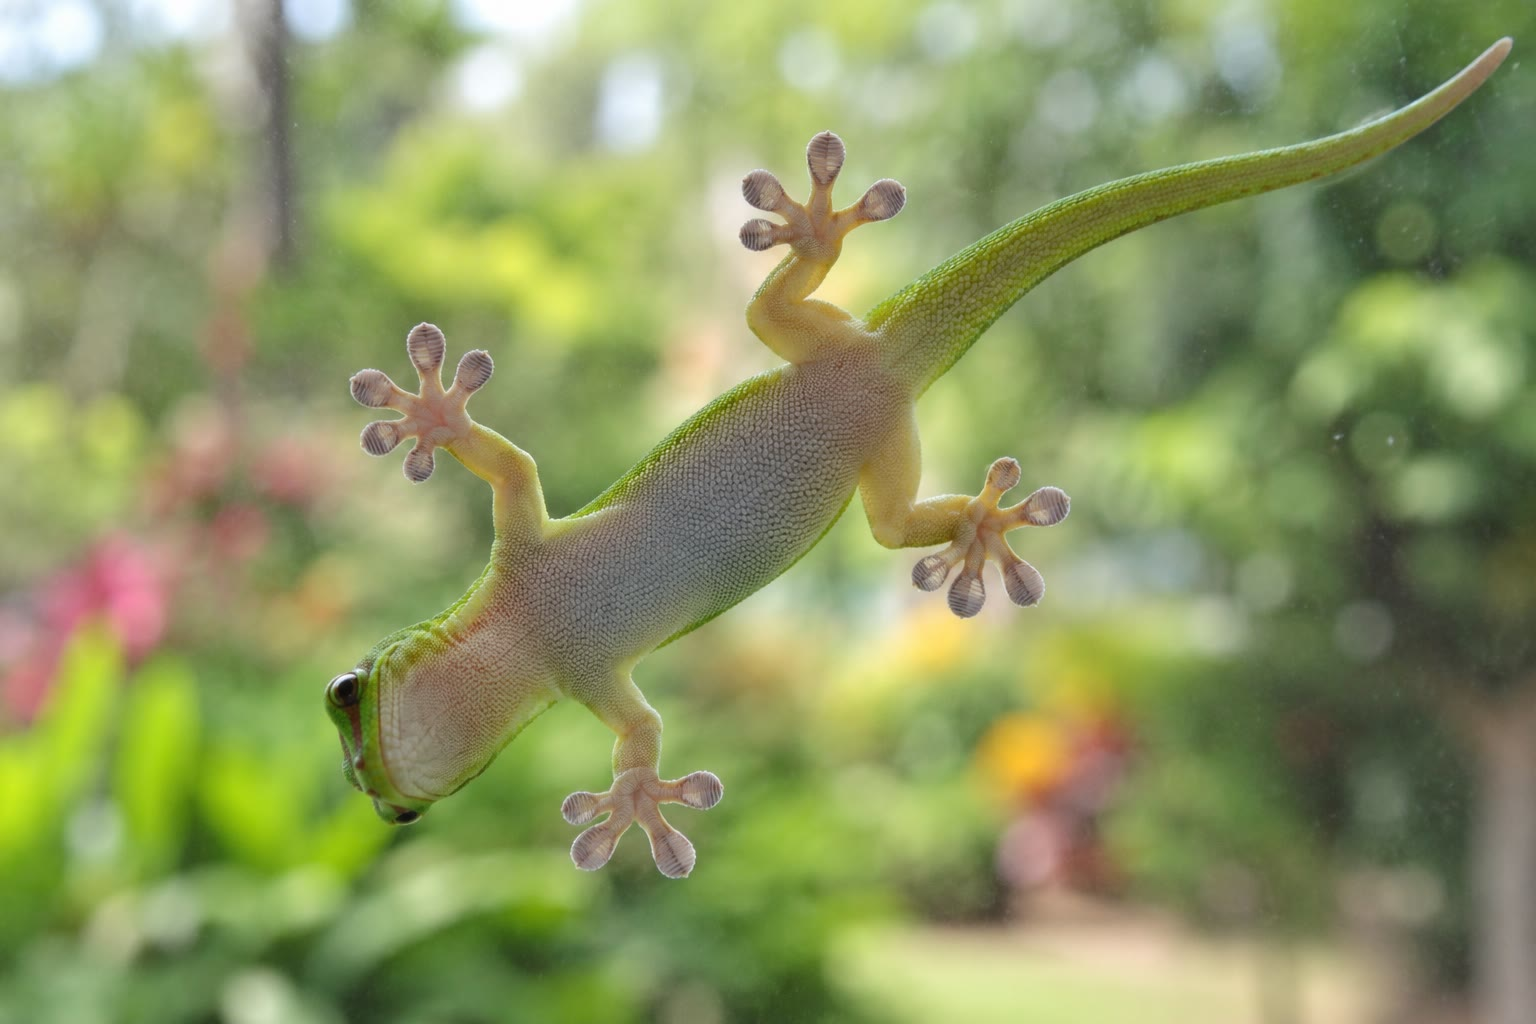
\includegraphics[width=0.5\linewidth]{images/book1/ai/g11-gecko-glass.jpg}

{\small Een gekko op een ruit: de kussentjes van zijn tenen houden zich
vast met krachten tussen \omterm{def:g7:atoms-and-molecules:molecule}{moleculen}.}
\end{omfigure}

\section{Elektronegativiteit}

\begin{definition}[Elektronegativiteit]\label{def:g11:polarity-and-cohesion:electronegativity}
De \emph{elektronegativiteit}\index{elektronegativiteit} van een element
geeft aan hoe sterk zijn \omterm{def:g7:atoms-and-molecules:atom}{atomen} in een \omterm{def:g7:atoms-and-molecules:molecule}{molecuul} de \omterm{def:g9:inside-the-atom:nucleus}{elektronen} van de
bindingen die ze delen naar zich toe trekken. Het is een getal zonder
eenheid; op de gebruikelijke schaal loopt het van ongeveer 0.8 tot
ongeveer 4.
\end{definition}

\begin{omfigure}
% ledger: en:H, en:Li, en:Be, en:B, en:C, en:N, en:O, en:F, en:Na, en:Mg, en:Al, en:Si, en:P, en:S, en:Cl, en:K, en:Ca
\omperiodictable[upto=20, f block=false, cell=0.9cm, values={H/2.20,
  Li/0.98, Be/1.57, B/2.04, C/2.55, N/3.04, O/3.44, F/3.98, Na/0.93,
  Mg/1.31, Al/1.61, Si/1.90, P/2.19, S/2.58, Cl/3.16, K/0.82, Ca/1.00},
  highlight={F,O,N,Cl}]

{\small \omterm{def:g11:polarity-and-cohesion:electronegativity}{Elektronegativiteiten} van de eerste twintig elementen
(schaal van Pauling; voor helium, neon en argon, die hier geen bindingen
vormen, is er geen gegeven). Gemarkeerd: de vier meest elektronegatieve.}
\end{omfigure}

\begin{proposition}[Trends in de tabel]\label{prop:g11:polarity-and-cohesion:trends}
% ledger: en:F, en:Li, en:Cl, en:K
De \omterm{def:g11:polarity-and-cohesion:electronegativity}{elektronegativiteit} neemt langs een periode toe van links naar rechts
en neemt in een groep af van boven naar beneden. Fluor (3.98) is het meest
elektronegatieve element; de \omterm{def:g10:electron-shells:family}{alkalimetalen} zijn het minst
elektronegatief (lithium 0.98, kalium 0.82).
\end{proposition}

\begin{proof}
Lees af in de tabel: langs periode 2, $0.98 < 1.57 < 2.04 < 2.55 < 3.04 <
3.44 < 3.98$; naar beneden in \omterm{def:g9:periodic-table-first-look:period}{groep} 17 staat fluor $3.98$ boven chloor
$3.16$; naar beneden in \omterm{def:g9:periodic-table-first-look:period}{groep} 1, $2.20$, $0.98$, $0.93$, $0.82$. (Waarom
dat zo is, legt het deel voor het eerste universiteitsjaar uit.)
\end{proof}

\begin{history}[De schaal van Pauling, 1932]
De scheikundige Linus Pauling stelde in 1932 de eerste
elektronegativiteitsschaal op, uit de energieën van bindingen tussen
verschillende \omterm{def:g7:atoms-and-molecules:atom}{atomen}. Hij gaf fluor de grootste waarde, en de schaal die
in dit hoofdstuk gebruikt wordt, is nog altijd naar hem genoemd.
\end{history}

\section{Polaire bindingen en polaire moleculen}

\begin{definition}[Polaire binding, partiële lading]\label{def:g11:polarity-and-cohesion:polar-bond}
Een \omterm{def:g10:lewis-and-shape:covalent-bond}{covalente binding} tussen twee \omterm{def:g7:atoms-and-molecules:atom}{atomen} met een verschillende
\omterm{def:g11:polarity-and-cohesion:electronegativity}{elektronegativiteit} is een \emph{polaire binding}\index{polaire binding}:
het gedeelde paar zit dichter bij het meest elektronegatieve \omterm{def:g7:atoms-and-molecules:atom}{atoom}. Dat
\omterm{def:g7:atoms-and-molecules:atom}{atoom} draagt een kleine negatieve \emph{partiële lading}\index{partiële lading},
geschreven als $\delta^-$, en het andere \omterm{def:g7:atoms-and-molecules:atom}{atoom} een even grote positieve
partiële lading, $\delta^+$.
\end{definition}

\begin{proposition}[Wanneer is een binding polair?]\label{prop:g11:polarity-and-cohesion:polar-bond}
% ledger: en:C, en:H, en:O, en:Na, en:Cl
Een binding tussen twee gelijke \omterm{def:g7:atoms-and-molecules:atom}{atomen} is niet polair. Tussen
verschillende \omterm{def:g7:atoms-and-molecules:atom}{atomen} geldt: hoe groter het verschil in
\omterm{def:g11:polarity-and-cohesion:electronegativity}{elektronegativiteit}, hoe polairder de binding; als vuistregel geldt een
verschil onder ongeveer 0.4 (zoals bij
\ce{C-H}, $2.55 - 2.20 = 0.35$) als apolair. Is het verschil heel groot
(zoals bij Na en Cl, $3.16 - 0.93 = 2.23$), dan worden de
\omterm{def:g9:inside-the-atom:nucleus}{elektronen} niet gedeeld maar overgedragen: de verbinding is ionair.
\end{proposition}

\begin{proof}
Aangenomen: het volgt uit de definitie van \omterm{def:g11:polarity-and-cohesion:electronegativity}{elektronegativiteit}, en de
grenzen zijn afspraken.
\end{proof}

\begin{definition}[Polaire en apolaire moleculen]\label{def:g11:polarity-and-cohesion:polar-molecule}
Een \omterm{def:g7:atoms-and-molecules:molecule}{molecuul} is een \emph{polair molecuul}\index{polair molecuul} als het
zwaartepunt van zijn positieve \omterm{def:g11:polarity-and-cohesion:polar-bond}{partiële ladingen} en dat van zijn
negatieve \omterm{def:g11:polarity-and-cohesion:polar-bond}{partiële ladingen} niet samenvallen; vallen ze samen, dan is het
een \emph{apolair molecuul}\index{apolair molecuul}.
\end{definition}

\begin{method}[Is een molecuul polair?]\label{met:g11:polarity-and-cohesion:polar}
\begin{enumerate}
  \item Teken de \omterm{def:g10:lewis-and-shape:lewis-structure}{lewisstructuur} en bepaal de vorm van het \omterm{def:g7:atoms-and-molecules:molecule}{molecuul}.
  \item Geef de \omterm{def:g11:polarity-and-cohesion:polar-bond}{polaire bindingen} aan met $\delta^+$ en $\delta^-$.
  \item Is er geen enkele \omterm{def:g11:polarity-and-cohesion:polar-bond}{polaire binding}, dan is het \omterm{def:g7:atoms-and-molecules:molecule}{molecuul} apolair.
        Anders kijk je naar de vorm: liggen de \omterm{def:g11:polarity-and-cohesion:polar-bond}{polaire bindingen}
        symmetrisch rond het midden, dan heffen hun effecten elkaar op
        en is het \omterm{def:g7:atoms-and-molecules:molecule}{molecuul} apolair; zo niet, dan is het polair.
\end{enumerate}
\end{method}

\begin{omfigure}
\begin{tikzpicture}[font=\small]
  % water
  \begin{scope}
    \node[aO] (o) at (0,0) {};
    \node[aH] (h1) at (-0.82,-0.6) {};
    \node[aH] (h2) at (0.82,-0.6) {};
    \begin{scope}[on background layer]
      \draw[bond] (o.center) -- (h1.center); \draw[bond] (o.center) -- (h2.center);
    \end{scope}
    \node[omThm] at (0,0.55) {$2\delta^-$};
    \node[omDef] at (-1.22,-0.5) {$\delta^+$};
    \node[omDef] at (1.22,-0.5) {$\delta^+$};
    \fill[omDef] (0,-0.6) circle (0.06);
    \fill[omThm] (0,0) circle (0.06);
    \draw[densely dotted, black!60] (-0.82,-0.6) -- (0.82,-0.6);
    \draw[<-, black!60] (0.08,-0.64) -- (1.55,-1.05) node[right, align=left,
      font=\footnotesize] {zwaartepunt\\ van de $\delta^+$};
    \node[align=center, anchor=north] at (0,-1.8) {water: gebogen, \textbf{polair}};
  \end{scope}
  % carbon dioxide
  \begin{scope}[xshift=6cm]
    \node[aO] (o1) at (-1.15,0) {};
    \node[aC] (c) at (0,0) {};
    \node[aO] (o2) at (1.15,0) {};
    \begin{scope}[on background layer]
      \draw[bond, double, double distance=1.6pt] (o1.center) -- (c.center);
      \draw[bond, double, double distance=1.6pt] (c.center) -- (o2.center);
    \end{scope}
    \node[omThm] at (-1.15,0.55) {$\delta^-$};
    \node[omThm] at (1.15,0.55) {$\delta^-$};
    \node[omDef] at (0,0.55) {$2\delta^+$};
    \draw[->, omProp, thick] (-0.25,-0.45) -- (-1.0,-0.45);
    \draw[->, omProp, thick] (0.25,-0.45) -- (1.0,-0.45);
    \node[align=center, anchor=north] at (0,-1.8) {koolstofdioxide: lineair,\\
      \textbf{apolair}};
  \end{scope}
\end{tikzpicture}

{\small In water legt de gebogen vorm het zwaartepunt van de positieve
\omterm{def:g11:polarity-and-cohesion:polar-bond}{partiële ladingen} (tussen de waterstofatomen) onder het zuurstofatoom:
het \omterm{def:g7:atoms-and-molecules:molecule}{molecuul} is polair. In koolstofdioxide trekken de twee \omterm{def:g11:polarity-and-cohesion:polar-bond}{polaire
bindingen} in tegengestelde richtingen (pijlen) en heffen ze elkaar op:
de zwaartepunten van de lading vallen samen op het koolstofatoom.}
\end{omfigure}


\begin{example}[Vier moleculen]\label{ex:g11:polarity-and-cohesion:four}
Waterstofchloride \ce{HCl} heeft één \omterm{def:g11:polarity-and-cohesion:polar-bond}{polaire binding} en is polair, met
chloor $\delta^-$. Ammoniak \ce{NH3}, een piramide van drie polaire
\ce{N-H}-bindingen, is polair, met stikstof $\delta^-$. Methaan \ce{CH4}
heeft alleen bijna apolaire \ce{C-H}-bindingen: apolair.
Tetrachloormethaan \ce{CCl4} heeft vier polaire \ce{C-Cl}-bindingen, maar
op de hoekpunten van een regelmatige tetraëder: hun effecten heffen
elkaar op en het \omterm{def:g7:atoms-and-molecules:molecule}{molecuul} is apolair.
\end{example}

\section{Vanderwaalsbindingen}

\begin{definition}[Vanderwaalsbinding]\label{def:g11:polarity-and-cohesion:van-der-waals}
Een \emph{vanderwaalsbinding}\index{vanderwaalsbinding} is een zwakke
aantrekking tussen naburige \omterm{def:g7:atoms-and-molecules:molecule}{moleculen}, die tussen alle \omterm{def:g7:atoms-and-molecules:molecule}{moleculen}
bestaat, polair of niet: de \omterm{def:g9:inside-the-atom:nucleus}{elektronen} van elk \omterm{def:g7:atoms-and-molecules:molecule}{molecuul} bewegen
voortdurend, en de tijdelijke ongelijke ladingen van het ene \omterm{def:g7:atoms-and-molecules:molecule}{molecuul}
trekken die van zijn buren aan. Tussen \omterm{def:g11:polarity-and-cohesion:polar-molecule}{polaire moleculen} geven de
blijvende \omterm{def:g11:polarity-and-cohesion:polar-bond}{partiële ladingen} nog een extra aantrekking.
\end{definition}


\begin{proposition}[Grotere moleculen trekken sterker aan]\label{prop:g11:polarity-and-cohesion:size}
\omterm{def:g11:polarity-and-cohesion:van-der-waals}{Vanderwaalsbindingen} worden sterker naarmate de \omterm{def:g7:atoms-and-molecules:molecule}{moleculen} groter zijn,
dus naarmate ze meer \omterm{def:g9:inside-the-atom:nucleus}{elektronen} hebben; tussen vergelijkbare \omterm{def:g7:atoms-and-molecules:molecule}{moleculen}
hebben de grotere het hogere smelt- en kookpunt.
\end{proposition}

\begin{proof}
Aangenomen: een grotere elektronenwolk is makkelijker te vervormen, dus
zijn tijdelijke ladingen zijn groter, en hij heeft meer contact met zijn
buren.
\end{proof}

\begin{example}[De halogenen]\label{ex:g11:polarity-and-cohesion:halogens}
% ledger: bp:F2, bp:Cl2, bp:Br2, bp:I2 (K values converted)
De \omterm{def:g7:atoms-and-molecules:molecule}{moleculen} \ce{F2}, \ce{Cl2}, \ce{Br2}, \ce{I2} zijn allemaal apolair
en steeds groter. Hun kookpunten stijgen mee:
\qty{-188}{\celsius}, \qty{-34}{\celsius}, \qty{59}{\celsius} en
\qty{184}{\celsius}. Bij kamertemperatuur zijn fluor en chloor gassen,
broom een vloeistof en jood een vaste stof.
\end{example}

\begin{remark}[De gekko]\label{rem:g11:polarity-and-cohesion:gecko}
Eén \omterm{def:g11:polarity-and-cohesion:van-der-waals}{vanderwaalsbinding} is piepklein, maar ze tellen op. De
teenkussentjes van een gekko zijn bedekt met een dicht tapijt van
microscopisch kleine haartjes, die zich elk weer splitsen in nog fijnere
uiteinden, die zo dicht bij het glas komen dat \omterm{def:g11:polarity-and-cohesion:van-der-waals}{vanderwaalsbindingen} over
een heel groot totaal oppervlak werken.
\end{remark}

\section{Waterstofbruggen}

\begin{definition}[Waterstofbrug]\label{def:g11:polarity-and-cohesion:hydrogen-bond}
Een \emph{waterstofbrug}\index{waterstofbrug} is een aantrekking tussen
een waterstofatoom dat gebonden is aan een heel elektronegatief \omterm{def:g7:atoms-and-molecules:atom}{atoom}
(stikstof, zuurstof of fluor), en daardoor een duidelijke $\delta^+$
draagt, en een \omterm{def:g10:lewis-and-shape:lone-pair}{vrij elektronenpaar} van een ander stikstof-, zuurstof- of
fluoratoom, vaak op een naburig \omterm{def:g7:atoms-and-molecules:molecule}{molecuul}. Je tekent haar als een
stippellijn, en de drie betrokken \omterm{def:g7:atoms-and-molecules:atom}{atomen} liggen bijna op een rechte lijn.
\end{definition}

\begin{omfigure}
\begin{tikzpicture}[font=\small]
  % central water molecule and four neighbours, H-bonds dashed
  \newcommand{\water}[4]{% name, x, y, rotation
    \begin{scope}[shift={(#2,#3)}, rotate=#4]
      \node[aO] (#1o) at (0,0) {};
      \node[aH] (#1a) at (-0.6,-0.45) {};
      \node[aH] (#1b) at (0.6,-0.45) {};
    \end{scope}
    \begin{scope}[on background layer]
      \draw[bond] (#1o.center) -- (#1a.center); \draw[bond] (#1o.center) -- (#1b.center);
    \end{scope}}
  \water{m}{0}{0}{0}
  \water{p}{-1.62}{-1.215}{0}
  \water{q}{1.62}{-1.215}{0}
  \water{r}{-1.435}{1.435}{-8.13}
  \water{s}{1.435}{1.435}{8.13}
  % H-bonds: m's H to p's O and q's O; r's and s's H to m's O
  \draw[dashed, omDef, thick] (ma) -- (po);
  \draw[dashed, omDef, thick] (mb) -- (qo);
  \draw[dashed, omDef, thick] (rb) -- (mo);
  \draw[dashed, omDef, thick] (sa) -- (mo);
\end{tikzpicture}

{\small \omterm{def:g11:polarity-and-cohesion:hydrogen-bond}{Waterstofbruggen} (gestippeld) rond een watermolecuul in vloeibaar
water: zijn twee waterstofatomen binden aan de zuurstofatomen van twee
buren, en de twee \omterm{def:g10:lewis-and-shape:lone-pair}{vrije elektronenparen} van zijn zuurstofatoom nemen de
waterstofatomen van twee andere op.}
\end{omfigure}


\begin{example}[Ethanol en propaan]\label{ex:g11:polarity-and-cohesion:ethanol}
% ledger: bp:C2H5OH, bp:C3H8 (K values converted)
Ethanol, \ce{CH3-CH2-OH} (\qty{46.0}{g/mol}), en propaan,
\ce{CH3-CH2-CH3} (\qty{44.0}{g/mol}), hebben \omterm{def:g7:atoms-and-molecules:molecule}{moleculen} van bijna dezelfde
grootte. Toch kookt ethanol bij \qty{78}{\celsius} en propaan bij
\qty{-42}{\celsius}. Ethanolmoleculen vormen met hun \ce{O-H}-groep
\omterm{def:g11:polarity-and-cohesion:hydrogen-bond}{waterstofbruggen} met elkaar; propaanmoleculen kunnen dat niet.
\end{example}

\section{De samenhang van vaste stoffen en vloeistoffen}

\begin{definition}[Moleculaire vaste stof]\label{def:g11:polarity-and-cohesion:molecular-solid}
Een \emph{moleculaire vaste stof}\index{moleculaire vaste stof} is een
vaste stof die bestaat uit \omterm{def:g7:atoms-and-molecules:molecule}{moleculen} die bij elkaar gehouden worden door
\omterm{def:g11:polarity-and-cohesion:van-der-waals}{vanderwaalsbindingen} en, waar dat kan, \omterm{def:g11:polarity-and-cohesion:hydrogen-bond}{waterstofbruggen}. IJs, vast jood
en suiker zijn moleculaire vaste stoffen.
\end{definition}

\begin{proposition}[Samenhang en faseovergang]\label{prop:g11:polarity-and-cohesion:cohesion}
Hoe sterker de aantrekking tussen de deeltjes van een stof, hoe hoger
haar smelt- en kookpunt. In volgorde van toenemende sterkte:
\omterm{def:g11:polarity-and-cohesion:van-der-waals}{vanderwaalsbindingen}, \omterm{def:g11:polarity-and-cohesion:hydrogen-bond}{waterstofbruggen}, en de aantrekking tussen de
\omterm{def:g9:ions:ion}{ionen} van een ionaire vaste stof.
\end{proposition}

\begin{proof}
Aangenomen: bij smelten en koken worden de deeltjes tegen deze
aantrekking in uit elkaar getrokken, wat meer energie kost, dus een
hogere temperatuur, als ze sterker is.
\end{proof}

\begin{example}[Drie vaste stoffen]\label{ex:g11:polarity-and-cohesion:three}
% ledger: mp:NaCl, mp:water
Natriumchloride, een ionaire vaste stof, smelt bij \qty{801}{\celsius};
ijs, bijeengehouden door \omterm{def:g11:polarity-and-cohesion:hydrogen-bond}{waterstofbruggen}, bij \qty{0}{\celsius}; vast
methaan, alleen bijeengehouden door \omterm{def:g11:polarity-and-cohesion:van-der-waals}{vanderwaalsbindingen} tussen kleine
\omterm{def:g7:atoms-and-molecules:molecule}{moleculen}, ver onder \qty{-150}{\celsius}.
\end{example}

\begin{omfigure}
\begin{tikzpicture}
\begin{axis}[width=0.6\linewidth, height=7cm, xmin=1.7, xmax=5.3,
    ymin=-190, ymax=120, xtick={2,3,4,5}, xlabel={periode},
    ylabel={kookpunt (\si{\celsius})}, axis lines*=left,
    ymajorgrids, grid style={gray!20}, tick label style={font=\small},
    label style={font=\small},
    legend style={font=\small, at={(1.02,0.5)}, anchor=west, draw=none},
    legend cell align=left]
  % ledger: bp:CH4, bp:SiH4, bp:GeH4, bp:NH3, bp:PH3, bp:AsH3, bp:SbH3, bp:H2O, bp:H2S, bp:H2Se, bp:HF, bp:HCl, bp:HBr, bp:HI (K values converted to degC)
  \addplot[thick, mark=*, black!70] coordinates {(2,-162.2) (3,-112) (4,-88.1)};
  \addplot[thick, mark=square*, omMeth] coordinates {(2,-33.4) (3,-87.8) (4,-62.5) (5,-18.4)};
  \addplot[thick, mark=triangle*, mark size=3pt, omThm] coordinates {(2,100.0) (3,-60.3) (4,-41.3)};
  \addplot[thick, mark=diamond*, mark size=3pt, omDef] coordinates {(2,19.6) (3,-85.1) (4,-66.4) (5,-35.1)};
  \legend{groep 14 (\ce{CH4} \dots), groep 15 (\ce{NH3} \dots),
    groep 16 (\ce{H2O} \dots), groep 17 (\ce{HF} \dots)}
  \node[font=\footnotesize, anchor=west] at (axis cs:2.05,100) {\ce{H2O}};
  \node[font=\footnotesize, anchor=west] at (axis cs:2.05,19.6) {\ce{HF}};
  \node[font=\footnotesize, anchor=west] at (axis cs:2.05,-33.4) {\ce{NH3}};
  \node[font=\footnotesize, anchor=north west] at (axis cs:2.05,-166) {\ce{CH4}};
\end{axis}
\end{tikzpicture}

{\small Kookpunten van de verbindingen van waterstof met de elementen van
de \omterm{def:g9:periodic-table-first-look:period}{groepen} 14 tot en met 17. In elke groep stijgen ze met de grootte van
het \omterm{def:g7:atoms-and-molecules:molecule}{molecuul}, behalve bij het eerste lid van de \omterm{def:g9:periodic-table-first-look:period}{groepen} 15, 16 en 17, dat
veel te hoog ligt: ammoniak, water en waterstoffluoride vormen
\omterm{def:g11:polarity-and-cohesion:hydrogen-bond}{waterstofbruggen}. (Waar de gebruikte bronnen geen waarde geven, staat er
geen punt.)}
\end{omfigure}

\begin{remark}[IJs en sneeuw]\label{rem:g11:polarity-and-cohesion:ice}
In ijs is elk watermolecuul via \omterm{def:g11:polarity-and-cohesion:hydrogen-bond}{waterstofbruggen} gebonden aan vier
buren, in een open netwerk van zeshoekige ringen. Dat netwerk laat meer
lege ruimte over dan vloeibaar water, waarin de bruggen voortdurend
breken en opnieuw ontstaan: ijs is minder dicht dan water en drijft. De
zesvoudige symmetrie van sneeuwkristallen weerspiegelt de zeshoekige
ringen van het netwerk.
\end{remark}

\begin{omfigure}
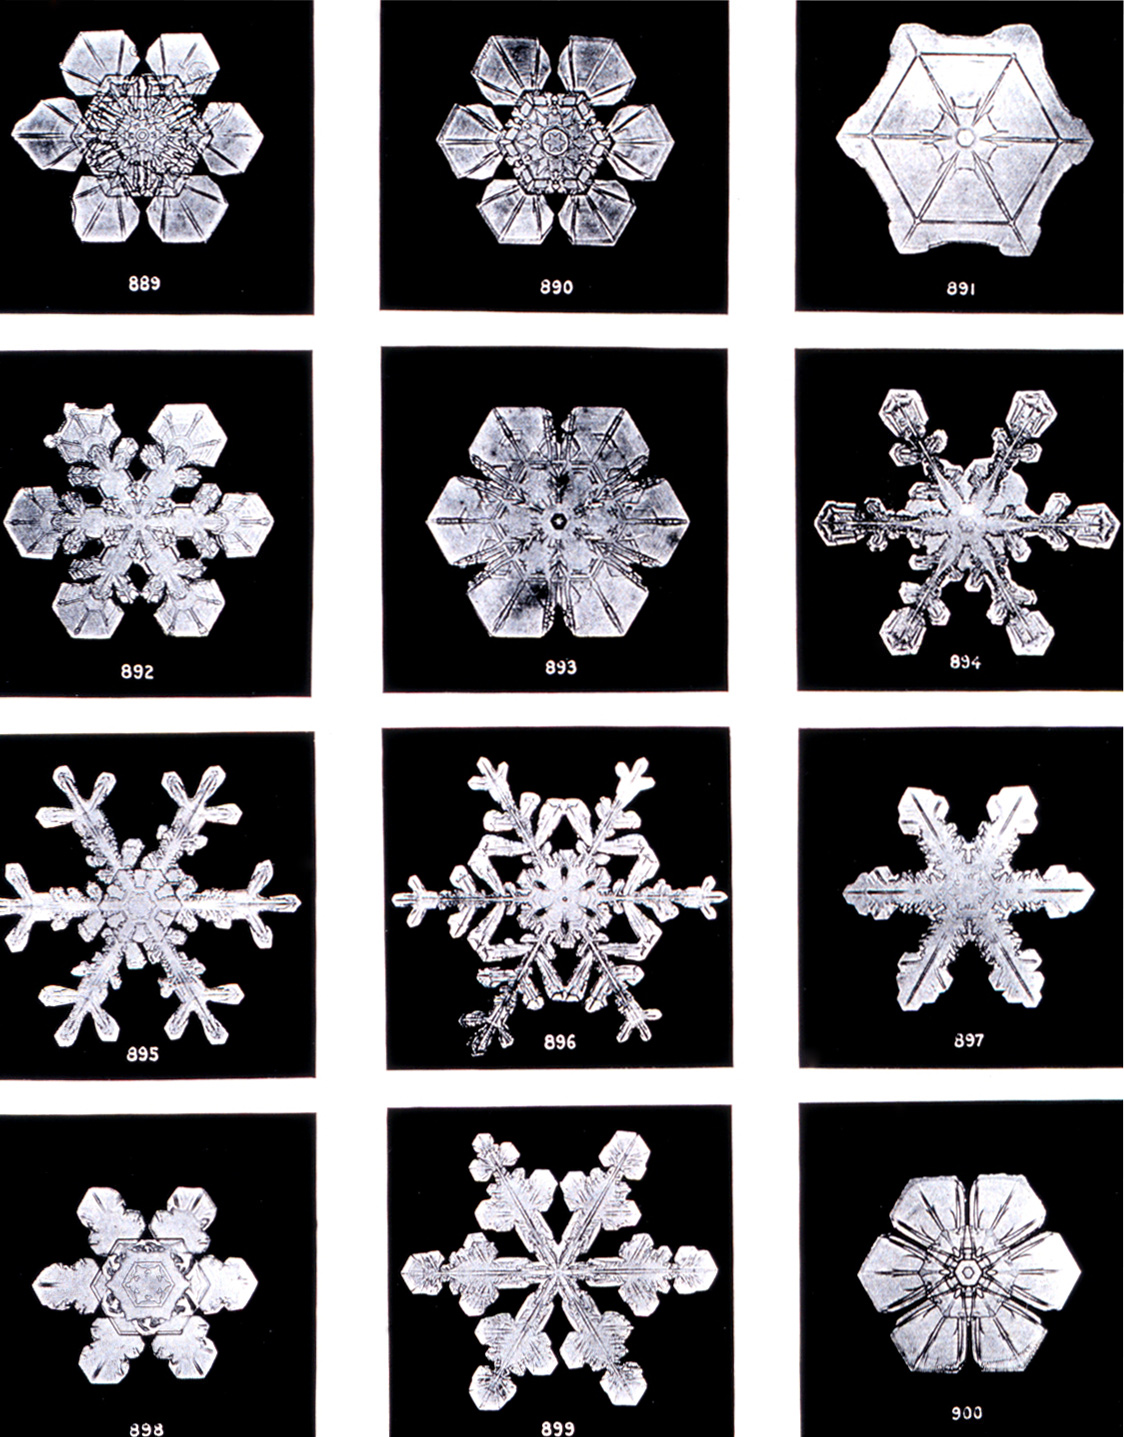
\includegraphics[width=0.36\linewidth]{images/book1/snowflakes.jpg}

{\small Sneeuwkristallen, begin twintigste eeuw gefotografeerd door Wilson
Bentley: elk ervan heeft zes takken.}
\end{omfigure}

\section{Oefeningen}


\begin{exercise}[$\star$]\label{exo:g11:polarity-and-cohesion:1}
Welk \omterm{def:g7:atoms-and-molecules:atom}{atoom} draagt in de bindingen \ce{H-Cl}, \ce{O-H} en \ce{C-O} de
\omterm{def:g11:polarity-and-cohesion:polar-bond}{partiële lading} $\delta^-$? Gebruik de tabel van \omterm{def:g11:polarity-and-cohesion:electronegativity}{elektronegativiteiten}.
\end{exercise}

\begin{exercise}[$\star$]\label{exo:g11:polarity-and-cohesion:2}
Welke van deze bindingen zijn polair: \ce{H-H}, \ce{C-H}, \ce{O-H},
\ce{N-H}, \ce{Cl-Cl}, \ce{C-Cl}? Geef voor elk het verschil in
\omterm{def:g11:polarity-and-cohesion:electronegativity}{elektronegativiteit}.
\end{exercise}

\begin{exercise}[$\star$]\label{exo:g11:polarity-and-cohesion:3}
Welk element is in elk paar het meest elektronegatief: stikstof of
fosfor; zuurstof of zwavel; koolstof of stikstof; natrium of magnesium?
Welke trend van de tabel illustreert elk paar?
\end{exercise}

\begin{exercise}[$\star$]\label{exo:g11:polarity-and-cohesion:4}
Welke van \ce{CH4}, \ce{NH3}, \ce{H2O} en \ce{HCl} kunnen \omterm{def:g11:polarity-and-cohesion:hydrogen-bond}{waterstofbruggen}
vormen tussen hun eigen \omterm{def:g7:atoms-and-molecules:molecule}{moleculen}? Leg uit.
\end{exercise}

\begin{exercise}[$\star$]\label{exo:g11:polarity-and-cohesion:5}
Is er aantrekking tussen de \omterm{def:g11:polarity-and-cohesion:polar-molecule}{apolaire moleculen} van methaan? Waarom is
methaan bij kamertemperatuur toch een gas?
\end{exercise}

\begin{exercise}[$\star\star$]\label{exo:g11:polarity-and-cohesion:6}
Zeg van elk \omterm{def:g7:atoms-and-molecules:molecule}{molecuul} of het polair is: dichloormethaan \ce{CH2Cl2}
(tetraëdrisch), tetrachloormethaan \ce{CCl4}, ammoniak \ce{NH3},
koolstofdioxide \ce{CO2}, boortrifluoride \ce{BF3} (een vlakke driehoek
met boor in het midden).
\end{exercise}

\begin{exercise}[$\star\star$]\label{exo:g11:polarity-and-cohesion:7}
Welk waterstofatoom in methanol, \ce{CH3-OH}, kan in een \omterm{def:g11:polarity-and-cohesion:hydrogen-bond}{waterstofbrug}
gegeven worden? Welk \omterm{def:g7:atoms-and-molecules:atom}{atoom} kan er een opnemen? Kunnen \omterm{def:g7:atoms-and-molecules:molecule}{moleculen} van
methanol en water \omterm{def:g11:polarity-and-cohesion:hydrogen-bond}{waterstofbruggen} met elkaar vormen? Teken er een.
\end{exercise}

\begin{exercise}[$\star\star$]\label{exo:g11:polarity-and-cohesion:8}
Leg uit waarom de kookpunten stijgen in de volgorde \ce{CH4} <
\ce{SiH4} < \ce{GeH4}.
\end{exercise}

\begin{exercise}[$\star\star$]\label{exo:g11:polarity-and-cohesion:9}
Welke groep laat in de grafiek van de kookpunten van de hydriden geen
afwijkende waarde zien voor haar eerste lid? Waarom niet?
\end{exercise}

\begin{exercise}[$\star\star$]\label{exo:g11:polarity-and-cohesion:10}
% ledger: en:H, en:Cl, en:Br, en:I, bp:HCl, bp:HBr, bp:HI
De bindingen \ce{H-Cl}, \ce{H-Br}, \ce{H-I} zijn steeds minder polair (de
\omterm{def:g11:polarity-and-cohesion:electronegativity}{elektronegativiteiten} van chloor, broom en jood zijn 3.16, 2.96 en
2.66), en toch stijgen de kookpunten: \qty{-85}{\celsius},
\qty{-66}{\celsius}, \qty{-35}{\celsius}. Welke aantrekking wint, en
waarom?
\end{exercise}

\begin{exercise}[$\star\star$]\label{exo:g11:polarity-and-cohesion:11}
Bij kamertemperatuur is chloor een gas en jood een vaste stof, hoewel
beide uit \omterm{def:g11:polarity-and-cohesion:polar-molecule}{apolaire moleculen} \ce{X2} bestaan. Leg uit.
\end{exercise}

\begin{exercise}[$\star\star\star$]\label{exo:g11:polarity-and-cohesion:12}
% ledger: bp:C2H5OH, bp:CH3OCH3, bp:C3H8
Ethanol \ce{CH3-CH2-OH}, methoxymethaan \ce{CH3-O-CH3} en propaan
\ce{CH3-CH2-CH3} hebben bijna dezelfde \omterm{def:g10:the-mole:molar-mass}{molaire massa}. Ze koken bij
\qty{78}{\celsius}, \qty{-25}{\celsius} en \qty{-42}{\celsius}. Welke
ervan zijn polair? Welke vormen \omterm{def:g11:polarity-and-cohesion:hydrogen-bond}{waterstofbruggen} tussen hun eigen
\omterm{def:g7:atoms-and-molecules:molecule}{moleculen}? Verklaar de volgorde.
\end{exercise}

\begin{exercise}[$\star\star\star$]\label{exo:g11:polarity-and-cohesion:13}
In ijs is elk watermolecuul via \omterm{def:g11:polarity-and-cohesion:hydrogen-bond}{waterstofbruggen} gebonden aan vier buren,
in een open netwerk; in vloeibaar water breekt het netwerk voortdurend en
stort het deels in. Leg uit waarom ijs op water drijft. Waarom is dat
belangrijk voor de vissen in een bevroren meer?
\end{exercise}

\begin{exercise}[$\star\star\star$]\label{exo:g11:polarity-and-cohesion:14}
Zet in volgorde van toenemend smeltpunt, en verklaar met de aantrekking
tussen de deeltjes: kaliumchloride \ce{KCl}, ijs \ce{H2O}, vast methaan
\ce{CH4}.
\end{exercise}

\begin{exercise}[$\star\star\star$]\label{exo:g11:polarity-and-cohesion:15}
% ledger: en:F, en:O, bp:HF, bp:H2O
Fluor is elektronegatiever dan zuurstof, dus een \ce{H-F}-binding is
polairder dan een \ce{O-H}-binding. Toch kookt water bij
\qty{100}{\celsius} en waterstoffluoride bij \qty{20}{\celsius}. Tel de
waterstofatomen die elk \omterm{def:g7:atoms-and-molecules:molecule}{molecuul} kan geven en de \omterm{def:g10:lewis-and-shape:lone-pair}{vrije elektronenparen}
waarmee het kan opnemen, en leg uit.
\end{exercise}

\section{Probleem: Waarom kookt water bij \texorpdfstring{\qty{100}{\celsius}}{100 graden Celsius}?}

\begin{problem}[{Weekendprobleem --- bij welke temperatuur zou water koken
zonder waterstofbruggen?}]
\label{pb:g11:polarity-and-cohesion:1}
% ledger: en:H, en:O, en:S, en:Se, bp:H2O, bp:H2S, bp:H2Se, bp:CH4, bp:SiH4, bp:GeH4, bp:HCl, bp:HBr, bp:HF, bp:NH3, bp:PH3, bp:AsH3
Zuurstof, zwavel en seleen staan in dezelfde groep van de tabel, en alle
drie vormen ze een verbinding met waterstof: \ce{H2O}, \ce{H2S},
\ce{H2Se}. In elke groep hydriden stijgen de kookpunten gewoonlijk met de
grootte van het \omterm{def:g7:atoms-and-molecules:molecule}{molecuul}. Water breekt die regel. Met hoeveel?

\medskip
\noindent\textbf{Deel I --- Drie \omterm{def:g7:atoms-and-molecules:molecule}{moleculen}.}
\begin{enumerate}
  \item Teken de \omterm{def:g10:lewis-and-shape:lewis-structure}{lewisstructuren} van \ce{H2O}, \ce{H2S} en \ce{H2Se}.
        Waarom lijken ze op elkaar?
  \item Bereken hun \omterm{def:g10:the-mole:molar-mass}{molaire massa's}.
  \item Bereken de verschillen in \omterm{def:g11:polarity-and-cohesion:electronegativity}{elektronegativiteit} van de bindingen
        \ce{O-H}, \ce{S-H} en \ce{Se-H} (zuurstof 3.44, zwavel 2.58,
        seleen 2.55, waterstof 2.20). Welke bindingen zijn duidelijk
        polair?
  \item Wat is de vorm van de drie \omterm{def:g7:atoms-and-molecules:molecule}{moleculen}? Zijn ze polair?
  \item Tel de \omterm{def:g9:inside-the-atom:nucleus}{elektronen} van elk \omterm{def:g7:atoms-and-molecules:molecule}{molecuul}. Welk heeft de sterkste
        \omterm{def:g11:polarity-and-cohesion:van-der-waals}{vanderwaalsbindingen}?
\end{enumerate}

\medskip
\noindent\textbf{Deel II --- \omterm{def:g11:polarity-and-cohesion:hydrogen-bond}{Waterstofbruggen}.}
\begin{enumerate}[resume]
  \item Welke van de drie verbindingen vormt \omterm{def:g11:polarity-and-cohesion:hydrogen-bond}{waterstofbruggen} tussen haar
        \omterm{def:g7:atoms-and-molecules:molecule}{moleculen}? Waarom de andere niet?
  \item Aan hoeveel \omterm{def:g11:polarity-and-cohesion:hydrogen-bond}{waterstofbruggen} kan één watermolecuul hoogstens
        meedoen? Teken ze.
  \item Welke aantrekking houdt de \omterm{def:g7:atoms-and-molecules:molecule}{moleculen} van waterstofsulfide in de
        vloeistof bij elkaar?
\end{enumerate}

\medskip
\noindent\textbf{Deel III --- De trend.}
\begin{enumerate}[resume]
  \item Waterstofsulfide kookt bij \qty{212.9}{K} en waterstofselenide
        bij \qty{-41.3}{\celsius}. Druk de eerste uit in graden Celsius
        ($\theta = T - 273.15$).
  \item Hoeveel stijgt het kookpunt van periode 3 (\ce{H2S}) naar periode
        4 (\ce{H2Se})?
  \item Waarom stijgt het?
  \item Bij welke temperatuur zou een ``normaal'' \ce{H2O} koken, als je
        aanneemt dat het kookpunt van periode 2 naar periode 3 evenveel
        stijgt?
  \item Test de methode op \omterm{def:g9:periodic-table-first-look:period}{groep} 14: \ce{SiH4} kookt bij
        \qty{-112}{\celsius} en \ce{GeH4} bij \qty{-88.1}{\celsius}.
        Voorspel het kookpunt van \ce{CH4} en vergelijk met het echte,
        \qty{-162}{\celsius}. Is de extrapolatie exact?
  \item Doe hetzelfde voor \omterm{def:g9:periodic-table-first-look:period}{groep} 17 (\ce{HCl} \qty{-85.1}{\celsius},
        \ce{HBr} \qty{-66.4}{\celsius}) en vergelijk met \ce{HF},
        \qty{19.6}{\celsius}.
\end{enumerate}

\medskip
\noindent\textbf{Deel IV --- Het verschil.}
\begin{enumerate}[resume]
  \item Water kookt echt bij \qty{100}{\celsius}. Hoe groot is het
        verschil tussen de echte en de geëxtrapoleerde waarde?
  \item Hetzelfde voor ammoniak, met \ce{PH3} \qty{-87.8}{\celsius} en
        \ce{AsH3} \qty{-62.5}{\celsius}; ammoniak kookt echt bij
        \qty{-33.4}{\celsius}.
  \item Zet water, waterstoffluoride en ammoniak op volgorde van de
        grootte van hun verschil, en verklaar de volgorde door
        \omterm{def:g11:polarity-and-cohesion:hydrogen-bond}{waterstofbruggen} te tellen.
  \item Zou water zonder \omterm{def:g11:polarity-and-cohesion:hydrogen-bond}{waterstofbruggen} bij kamertemperatuur een vaste
        stof, een vloeistof of een gas zijn? Wat zou dat betekenen voor de
        aarde?
  \item Waarom is het antwoord op vraag 12 maar een schatting?
  \item Geef het eindantwoord: bij ongeveer welke temperatuur zou water
        zonder \omterm{def:g11:polarity-and-cohesion:hydrogen-bond}{waterstofbruggen} koken?
\end{enumerate}
\end{problem}
